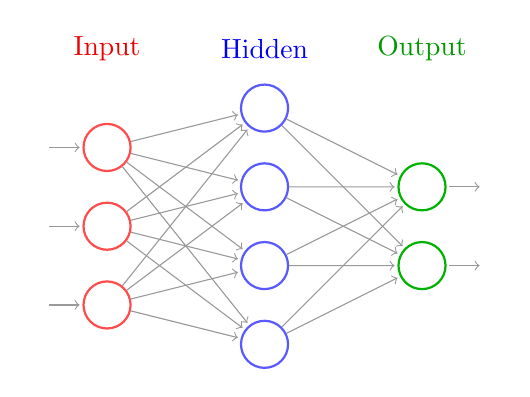
\begin{tikzpicture}[shorten >=1pt,->,draw=black!40, node distance=2cm]
    \tikzstyle{every pin edge}=[<-,shorten <=1pt]
    \tikzstyle{neuron}=[circle,minimum size=17pt,inner sep=0pt, line width=0.8]
    \tikzstyle{input neuron}=[neuron, draw=red!70];
    \tikzstyle{output neuron}=[neuron, draw=green!70!black];
    \tikzstyle{hidden neuron}=[neuron, draw=blue!65];
    \tikzstyle{annot} = [text width=4em, text centered]

    % Draw the input layer nodes
    \foreach \name / \y in {1,...,3}
    % This is the same as writing \foreach \name / \y in {1/1,2/2,3/3,4/4}
        \node[input neuron, pin=left: ] (I-\name) at (0,-\y) {};

    % Draw the hidden layer nodes
    \foreach \name / \y in {1,...,4}
        \path[yshift=0.5cm]
            node[hidden neuron, label=left:, label=right: ] (H-\name) at (2.0cm,-\y cm) {};

    % Draw the output layer nodes
    \foreach \name / \y in {1,...,2}
        \path[yshift=-0.5cm]
            node[output neuron, pin={[pin edge={->,shorten <=1pt}]right: }] (O-\name) at (4cm,-\y cm) {};

    % Connect every node in the input layer with every node in the
    % hidden layer.
    \foreach \source in {1,...,3}
        \foreach \dest in {1,...,4}
            \path (I-\source) edge (H-\dest);

    % Connect every node in the hidden layer with the output layer
    \foreach \source in {1,...,4}
        \foreach \dest in {1,...,2}
            \path (H-\source) edge (O-\dest);

    % Annotate the layers
    \node[annot,above of=H-1, node distance=0.75cm, color=blue!95!black] (hl) {Hidden};
    \node[annot,left of=hl, color=red!93!black] {Input};
    \node[annot,right of=hl, color=green!60!black] {Output};
\end{tikzpicture}

